\subsection{Private chain}

Private chain comprises of two main data structures:
\begin{itemize}
\item Merkle tree which consists of private blocks.
\item Indexed SQL database. The database stores links to transactions in the Merkle tree, indexed by tuples $(studentId, studentGrades)$.
\end{itemize}

The structure of the private block is shown in Figure \ref{fig:privateblocks}. The block consists of a public \textit{header} that the Educators relay to the Witnesses, and the private \textit{body} that remains in the educational institute until it receives a data disclosure request.

\begin{figure}[ht]
\centering
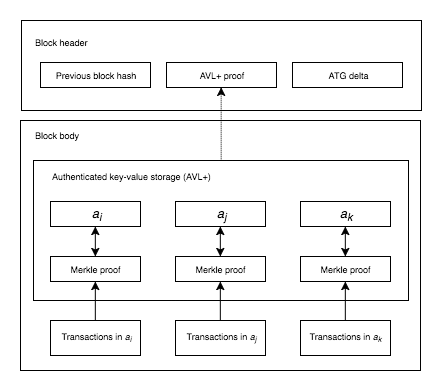
\includegraphics[width=0.8\textwidth]{private-blocks}
\caption{Private block structure}
\label{fig:privateblocks}
\end{figure}

During the educational process the Educators emit atomic \textit{private transactions}. These tansactions represent the modifications to the journal of academic achievements (thus, making a transaction means appending the data to the journal). The transactions can be of the following types:
\begin{itemize}
\item student enrolls in a course;
\item student gets an assignment;
\item student submits an assignment;
\item student gets a grade for an assignment;
\item student gets a final grade for the course.
\end{itemize}

The first two types should be intiated by a student, and should include student's signature to prevent spam from partially-honest educator.
The structure of the transaction is shown in Fugure \ref{fig:private-transactions}.

Let us denote an $i$-th transaction in a block as $T_{priv}^i$. The Educators group the transactions that occured during the current block time slot, and construct a Merkle tree \cite{merkle1989certified} for these journal modifications:
\begin{equation}
M_{priv} = \MerkleTree(T_{priv}^i)
\end{equation}

\begin{figure}[ht]
\centering
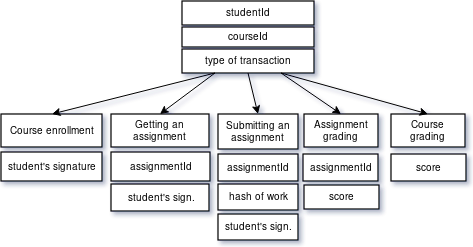
\includegraphics[width=0.8\textwidth]{private-transactions}
\caption{Transaction structure}
\label{fig:private-transactions}
\end{figure}



The Educator's private block body comprises an ordered set of Merkle-authenticated transactions. These transactions are indexed so that the Educator can quickly find a particular transaction that satisfies some predicate.

The private block header consists of the transactions Merkle root along with the previous block hash and the information on the Activity Type Graph modifications (ATG delta). The \textit{ATG delta} part allows the Educators to inform the Witnesses and the Archivists of the modifications to the courses they teach.

After the end of the block time slot, an Educator signs the block header and submits it to the Witnesses so that the private transactions can be confirmed by the public chain. Thus, the private blocks form a publicly verifiable chain of events, grouped according to the activity type.
